\section{Basismodell}
\label{subsubsec:Basismodel}
Ein Basismodell ist im Grundlegenden ein einfaches Modell, das als Referenz in einem ML-Projekt dient. Seine Hauptfunktion besteht darin, die Ergebnisse trainierter Modelle in einen Kontext zu setzen. Basismodelle sind normalerweise wenig komplex und können nur geringe Vorhersagekraft haben. Trotzdem ist ihre Einbeziehung aus verschiedenen Gründen notwendig \cite{Nair.04.04.2022}.
\newline
\newline
Einerseits dient das Basismodell dazu, einen initialen Einstieg in die Modellierung zu ermöglichen, dessen Ergebnisse anschließend mittels der zuvor ausgewählten Metrik evaluiert werden können. Hierbei wird ein vollständiger Workflow in vergleichsweise kurzer Zeit geschaffen. Andererseits fungiert das Basismodell als Referenzpunkt, welcher durch weitere Modelle übertroffen werden soll. Ein beispielhaftes Szenario für ein solches Basismodell könnte ein Empfehlungssystem für Filme sein, bei dem stets die aktuell beliebtesten Filme auf der Plattform angeboten werden.
\newline
\newline
Im vorliegenden Kontext besteht das Basismodell darin, vier zufällige Hotels aus dem Gesamtdatensatz zu extrahieren und diese als ähnlich zu betrachten. Mit dem Basismodell, welches vier zufällige Hotels liefert, sieht die Evaluation wie folgt aus:

\begin{figure}[h]
    \centering
    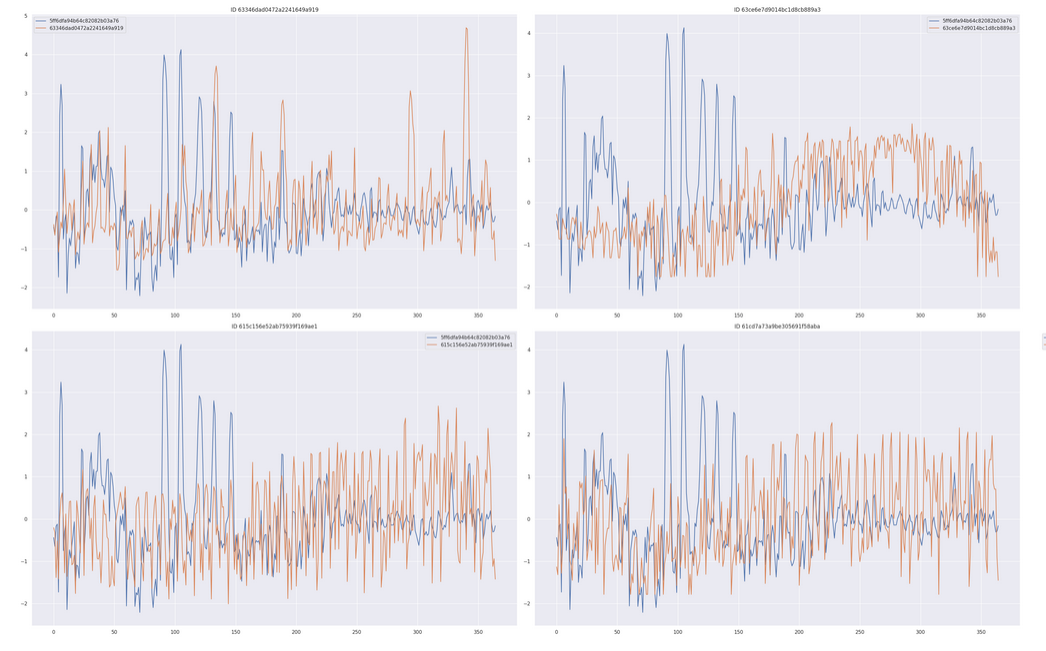
\includegraphics[width=1\textwidth, center]{basismodel_1.png}
    \caption[Basismodell Ergebnisse der RevPAR-Verläufe]{Basismodell Ergebnisse der RevPAR-Verläufe}
    \label{img:basismodell_1}
\end{figure}

\begin{figure}[h]
    \centering
    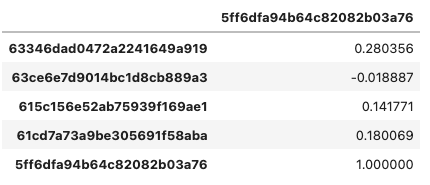
\includegraphics[width=0.5\textwidth, center]{basismodel_2.png}
    \caption[Basismodell Ergebnisse der RevPAR-Korrelationen]{Basismodell Ergebnisse RevPAR-Korrelationen}
    \label{img:basismodell_2}
\end{figure}

In den Abbildungen \ref{img:basismodell_1} und \ref{img:basismodell_2} sind die Ergebnisse für das Hotel mit der Identifikationsnummer \emph{5ff6dfa94b64c82082b03a76} im Zusammenhang mit dem Basismodell ersichtlich. Sowohl Abbildung \ref{img:basismodell_1} als auch Abbildung \ref{img:basismodell_2} verdeutlichen, dass die vier Hotels, welche vom Basismodell ausgewählt wurden, keine deutliche Ähnlichkeit aufweisen. Des Weiteren zeigt Abbildung \ref{img:basismodell_2} eindeutig, dass das angestrebte Ziel, ein Hotel mit einem Korrelationswert von mindestens 0,8 zu identifizieren, nicht erreicht wurde. Infolgedessen hat das Basismodell die entsprechende Anforderung nicht erfüllt.

